\section{实验结果}

\subsection{生成图像}

图~\ref{fig:input-pair} 展示程序实际使用的左右输入图像；图~\ref{fig:stereo-results}
从左至右给出归一化视差图、有效区域掩码和相对深度可视化。所有图片均直接引用
\codepath{task2/results/} 下的程序输出。

\begin{figure}[H]
  \centering
  
\includegraphics[width=0.48\linewidth]{../results/left.png}\hfill
  
\includegraphics[width=0.48\linewidth]{../results/right.png}
  \caption{OpenCV 官方 aloe 双目输入图（左：`aloeL.jpg`，右：`aloeR.jpg`）。}
  \label{fig:input-pair}
\end{figure}

\begin{figure}[H]
  \centering
  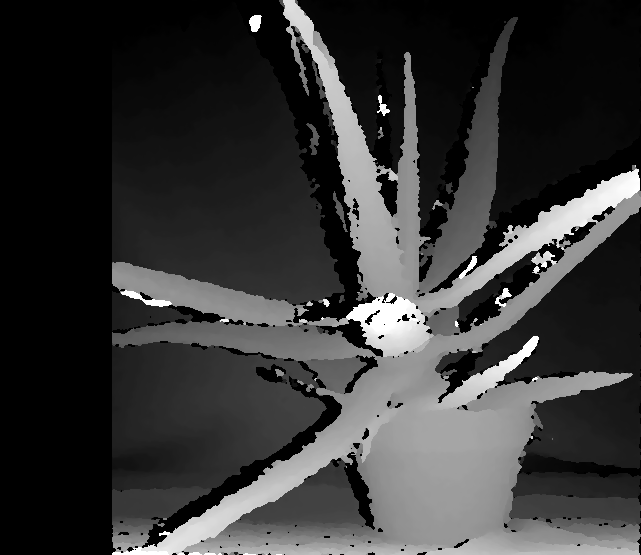
\includegraphics[width=0.31\linewidth]{../results/disparity.png}\hfill
  
\includegraphics[width=0.31\linewidth]{../results/valid_mask.png}\hfill
  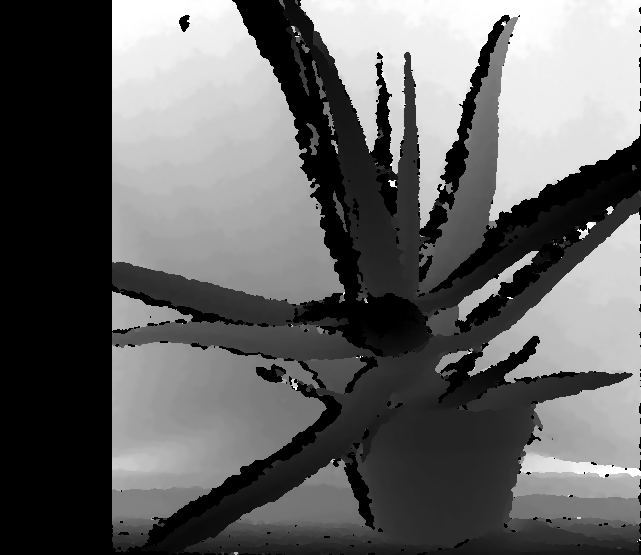
\includegraphics[width=0.31\linewidth]{../results/depth_proxy.png}
  \caption{程序生成的结果图（从左至右）：归一化视差图、有效视差掩码和任意尺度相对深度图。}
  \label{fig:stereo-results}
\end{figure}

\subsection{真实运行结果}

统计直接读取程序生成的 \codepath{disparity_raw.npy} 和
\codepath{depth_proxy.npy}，数组尺寸为 $555\times641$，总像素数为 $355755$。
在有限且满足 $d>15$ 的视差像素中，有 $261378$ 个有效像素，占总像素的
$73.4713\%$。表~\ref{tab:result-statistics} 汇总了真实运行结果。

\begin{table}[H]
  \centering
  \caption{OpenCV aloe 样例的真实运行结果统计}
  \label{tab:result-statistics}
  \begin{tabular}{ll}
    \toprule
    指标 & 实测值 \\
    \midrule
    原始图像尺寸 & $1282\times1110$ \\
    匹配图像尺寸 & $641\times555$ \\
    浮点数组尺寸 & $555\times641$ \\
    总像素 & $355755$ \\
    有效视差像素 & $261378$ \\
    有效视差像素比例 & $73.4713\%$ \\
    有效视差范围 & $16.000$--$105.875$~px \\
    相对深度范围 & $0.0094451$--$0.0625$（任意尺度） \\
    公式核验误差 $\max|z-1/d|$ & $0.0$ \\
    \bottomrule
  \end{tabular}
\end{table}

\subsection{结果分析与边界}

视差图和相对深度图保留了叶片、花盆和背景的主要结构，说明固定参数的 StereoSGBM
已经产生有效匹配。约 $26.5287\%$ 的像素未通过有效视差筛选，可能与遮挡、纹理
不足或左右图像中的匹配歧义有关；这些区域不能解释为可靠深度。

视差较低的有效像素范围为 $16.000$--$23.750$~px，其相对深度代理中位数为
$0.043127$；视差较高的有效像素范围为 $65.750$--$105.875$~px，其中位数为
$0.014172$。这与 $\mathrm{depth\_proxy}=1/d$ 一致：较大视差对应较小代理深度，
表示相对更近；较小视差对应较大代理深度，表示相对更远。

`aloeGT.png` 如被使用，只能作为官方视差参考图，不能作为相机标定或米制深度真值。
由于当前 aloe 图像对缺少经核验的 $f$、$B$ 和 $\mathbf{Q}$，本实验不能输出米、厘米
等物理单位的绝对深度或带物理尺度的三维点云。
